\subsection*{a}
Said $N(t)$ the number of atoms present at time $t$, the radioactive decay law states that
\begin{equation}
    \mathcal{A} = -\frac{dN}{dt} = \lambda N
    \label{eq:decay_law}
\end{equation}
where $\lambda$ is called the decay constant. \\
By integrating it in time one obtains 
\begin{equation}
    N(t) = N_0 \, e^{-\lambda t}
    \label{eq:decay_chain_first_atom}
\end{equation}
Now if we consider a chain decay of the type $A \rightarrow B \rightarrow C$ with initial conditions 
\begin{equation*}
    N_A(t=0) = N_0 \qquad N_B(t=0) = N_C(t=0) = 0
\end{equation*}
one can immediately obtain the number of $A$ atoms as a function of time by applying \ref{eq:decay_law}
\begin{equation*}
    N_A(t) = N_0 e^{-\lambda_A t}
\end{equation*}
To study the number of atoms of type $B$ one has to take account of two factors: the number of "created" atoms by means of $A$'s decay, and
the number of atoms decayed into $C$. This means that the radioactive law reads 
\begin{equation*}
    \frac{dN_B(t)}{dt} = -\lambda_B N_N(t) + \lambda_A N_{A \to B}(t)
\end{equation*}
where the first term on the right side member represents the $B$'s decay and the the last term 
takes account of the number of $B$'s obtained by $A$'s decay. \\
One can now substitute \ref{eq:decay_chain_first_atom} obtaining 
\begin{equation*}
    \frac{dN_B(t)}{dt} + \lambda_B N_B(t) =  \lambda_A N_0 \, e^{-\lambda_A t}
\end{equation*}
The general solution of this differential equation is 
\begin{equation*}
    N_B(t) = e^{-A(t)} \ \left(N_B(0) + \int_0^t \lambda_A N_0 e^{-\lambda_A s} e^{A(s)} \, ds \right)
\end{equation*}
where $A(s) = \lambda_B \int dt = \lambda_B t$. Hence
\begin{gather*}
N_B(t) = \lambda_A e^{-\lambda_B t} \ \int_0^t N_0 e^{-(\lambda_A - \lambda_B) s} \, ds 
= \frac{N_0 \lambda_A \, e^{-\lambda_B t}}{\lambda_A - \lambda_B} \ \left(1 - e^{-(\lambda_A - \lambda_B) t}\right) = \\
= N_0 \, \lambda_A \, \frac{e^{-\lambda_A t} - e^{-\lambda_B t}}{\lambda_B - \lambda_A}
\end{gather*}

\subsubsection*{b}
Let us consider the single-decay law 
\begin{equation*}
    N(t) = N_0 e^{-\lambda t}
\end{equation*}
One can notice here that $\lambda$'s physical units are inverse of time. The time $t_{1/2}$ is defined as the time necessary to halve the number of atoms fro $N_0$. 
This can be found by imposing $N(t) = N_0/2$ and solving for $t$ one obtains 
\begin{equation*}
    t_{1/2} = \frac{1}{\lambda} \, \log 2 \equiv \tau \log 2
\end{equation*}
where I introduced the mean lifetime $\tau \equiv 1/\lambda$. This last term, which has units of time, has a particular meaning. To understand this, one can first think 
of 
\begin{equation*}
    p(t) = \frac{N(t)}{\int N(t) \, dt}
\end{equation*} 
as a probability distribution function related to the probability of a particle to decay. One can then calculate the expected lifetime of such particle
\begin{equation*}
    \left\langle t \right\rangle = \frac{\int t N(t) \, dt}{\int N(t) \, dt} = \frac{\int_0^{\infty} te^{-\lambda t} \, dt}{\int_0^{\infty} e^{-\lambda t}} = \frac{1}{\lambda}
\end{equation*}
and it is exactly $\tau$. \\
Another interesting quantity is the natural decay width $\Gamma$. One can make plot the probability of a decay to occur as function of the decaying particle's energy: this function is peaked around
a most probable value $E_0$ with a distribution described by the Breit Wigner formula. The half width at half maximum of this distribution is the factor $\Gamma$ which has units of energy and is related to the average 
lifetime of the particle trough the relation
energy-time uncertainty relation
\begin{equation*}
    \Delta E \cdot \Delta t \approx \frac{\hbar}{2}
\end{equation*}
which in this particular case reads
\begin{equation*}
    \frac{\Gamma}{2} \cdot \tau \approx \frac{\hbar}{2}
\end{equation*}
or 
\begin{equation*}
    \tau \approx \frac{\hbar}{\gamma}
\end{equation*}

\subsubsection*{c}
$1mCi = 37MBq$. Taking the solution
\begin{equation*}
    N_1(t) = N_0 \, e^{-\lambda t}
\end{equation*}
and imposing $\mathcal{A}(t=0) = -\frac{dN_1(t)}{dt}|_{t=0} = 37MBq$ one obtains
\begin{equation*}
    N_0 = \frac{37 MBq}{\lambda} \simeq 29689798324
\end{equation*}
In this exercise I found some ambiguity with the definition of the activity in a decay chain. In fact, for a single decay, it is always true that 
\begin{equation}
    \frac{dN}{dt} = - \lambda N
    \label{eq:decay_law}
\end{equation}
hence one can calculate the activity both as $-\frac{dN}{dt}$ or $-\lambda N$. But when it comes to 
decay chains, it is not anymore true that for each species a relation as \ref{eq:decay_law} sussists, hence there are two possible definitions of the activity. Marting and Shaw (chapter 1.6.4 third edition)
defines tha activity as $\mathcal{A} = -\frac{dN}{dt}$, but other sources, such as \href{https://en.wikipedia.org/wiki/Radioactive_decay#Rates}{this}, use $\mathcal{A} = -\lambda N$ as definition. I chose to attach to the latter.
\subsection*{d}
\begin{figure}[htbp]
    \centering
    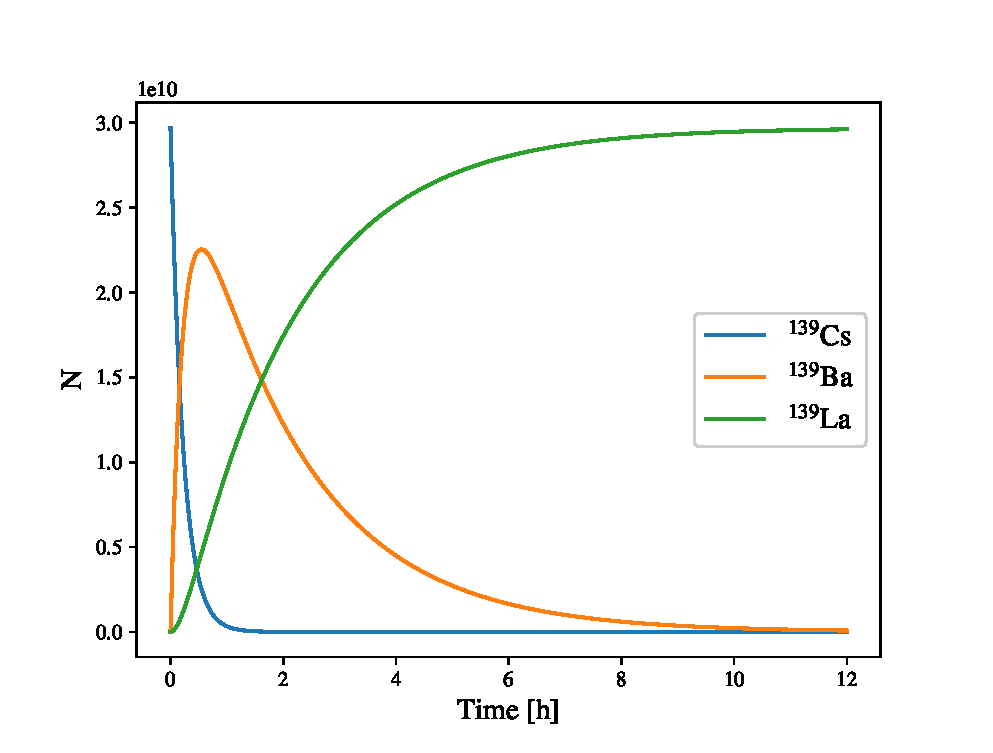
\includegraphics[scale=0.8]{ex7/decay.eps}
    \caption{Number of atoms as a function of time in the decay chain}
    \label{fig:decay_chain}
\end{figure}

\begin{figure}[htbp]
    \centering
    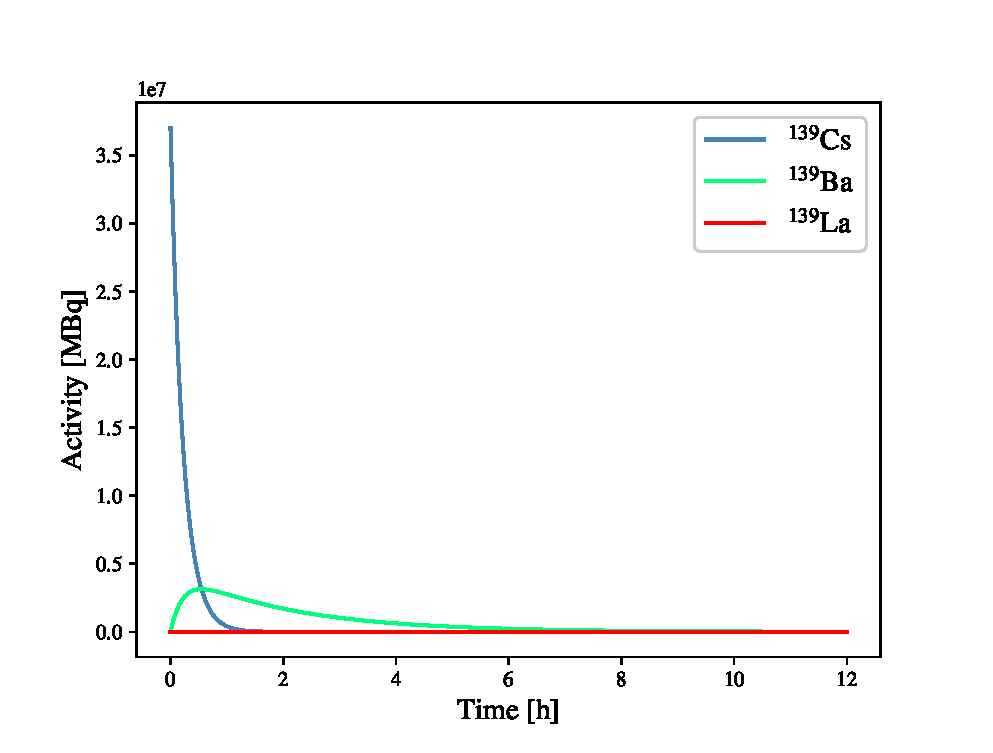
\includegraphics[scale=0.8]{ex7/decay_activities.eps}
    \caption{Activities as a function of time in the decay chain}
    \label{fig:decay_chain_activities}
\end{figure}

Figures \ref{fig:decay_chain} and \ref{fig:decay_chain_activities} report respectively
the number of atoms and the activities as functions of time. Of course at time $t=0$ the only present nuclei are $^{139}$Cs, and as the time passes 
the number of $^{139}$Cs nuclei decreases, while the two other elements start forming in chain. The activity of the first reaction is proportional to the 
the number of atoms of $^{139}$Cs, hence it is logical that the maximum activity of the first reaction is at the beginning of the simulation. For what concerns
$^{139}$Ba, the activity grows as more $^{139}$Ba atoms are produced but a certain point the rate of production of $^{139}$La overcomes the rate of decay of $^{139}$Cs,
and the $^{139}$Ba activity starts decreasing. Finally, the activity of $^{139}$La is always $0$ because no decays are observed

\subsubsection*{e}
The maximum activity of $^{139}$Ba is registered after $33$ minutes, with a maximum value of $3.1391~MBq = 0.0848~mCi$.

\subsubsection*{f}
The activities of $^{139}$Cs and $^{139}$Ba become equal after $0.33$ minutes (see script below), that is in the peak of the activity of  $^{139}$Ba.